\chapter{Problemak.}

\section{Sarrera.}

\section{Pendulu bikoitza.}

Planoan pendulu bikoitzaren problema era honetan definitzen da: $m_1$,$m_2$ masadun bi pendulu eta $l_1$, $l_2$ luzerako makilez (masa gabekoak kontsideratuko ditugunak) elkar lotuta. Penduluen aldagai-egoerak bi angelu ($\Theta_1$,$\Theta_2$) eta dagokion momentuak ($P_1$,$P_2$) dira.


\begin{figure} [h]
\centerline{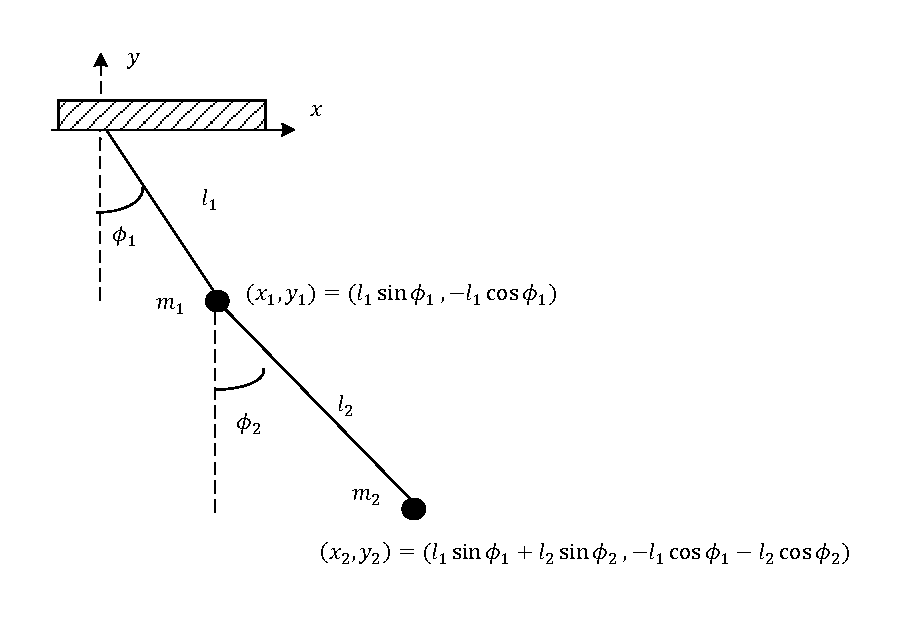
\includegraphics [width=10cm, height=8cm] {DoublePendulum}}
\caption{Pendulu bikoitza.}
\label{fig:41}
\end{figure} 

\subsection{Ekuazioak.}

\paragraph*{Hamiltondarra.}

\begin{equation*}
q=(\Theta_1,\Theta_2) \ \ , \ \ p=(P_1,P_2) \ \ , 
\end{equation*}

\begin{equation*} \label{eq:2}
H(q,p)= \bigg(\frac {C1 \ P_1^2 + C2 \ P_2^2 + 
 C3 \ P_1 \ P_2 \ \cos(\Theta_1 - \Theta_2)} {
 (C4 + C5 \ \sin^2 (Q_1 - Q_2))}\bigg)\\
       -C6 \ \cos(\Theta_1)-\ C7 \ \cos(\Theta_2), 
\end{equation*}

\paragraph*{}
     $C1 = l_2^2*m_2$,\\
     $C2 = l_1^2*(m_1 + m_2)$,\\
     $C3 = -2*l_1*l_2*l_2$,\\
     $C4 = 2*l_1^2*l_2^2*m_2*m_1$,\\
     $C5 = 2*m_1^2*l_2^2*m_2^2$,\\
     $C6 = g*l_1*(m_1 + m_2)$,\\
     $C7 = g*l_2*m_2$.


\paragraph*{Ekuazio diferentzialak.}

\begin{equation*}
\dot{\Theta_1}= \frac {2*C1*P1+C3*\cos(Q1-Q2)*P2}{aux1},
\end{equation*}

\begin{equation*}
 \ \ \dot{\Theta_2}= \frac{(2*C2*P2+C3*\cos(Q1-Q2)*P1)}{aux1},
\end{equation*}

\begin{equation*}
\dot{P1}=-(aux4+C6*\sin(Q1)), 
\end{equation*}

\begin{equation*}
\dot{P1}=(aux4-C7*\sin(Q2)), 
\end{equation*}

\paragraph*{}
$aux1=C4+C5*\sin(Q1-Q2)*\sin(Q1-Q2)$, \\
$aux2=C3*\cos(Q1-Q2)$,\\
$aux3=2*C5*\sin(Q1-Q2)*\cos(Q1-Q2)$,\\
$aux4=\frac{(-1/aux1^2)*(C1*P1^2+C2*P2^2+P1*P2*aux2)*aux3)-(C3*P1*P2*\sin(Q1-Q2))}{aux1}.$ 


\subsection{Hasierako balioak.}

\paragraph*{\textbf{Sistemaren parametroak}.} 
Gure esperimentuetarako honako parametroak kontsideratuko ditugu,
\begin{equation*} \label{eq:17}
g=9.8 \ \frac{m}{sec^2}\,\ \ l_1=1.0 \ m \ , \ l_2=1.0 \ m\ , \ m_1=1.0 \ kg\ , \ m_2=1.0 \ kg
\end{equation*} 

\paragraph*{\textbf{Hasierako balioak}.}
Pendulu bikoitza izaera kaotikoa duen sistema ez-lineala da. Zentzu honetan bi hasierako balio ezberdin kontsideratu ditugu \cite{Papadrakakis}:

\begin{enumerate}
   \item Hasierako balio ez-kaotikoak:   
   \ $q(0)=(1.1, 0)$ \ , \ $p(0)=(0,2.7746)$.    
   \item Hasierako balio kaotikoak: \ \ \ \ \    
   $q(0)=(0,0)$ \ , \ \ \  $p(0)=(0,3.873)$.
\end{enumerate}


\subsection{Kodeak.}

Mathematican DoublePendulum.m paketean honako funtzioak inplementatu ditugu:

\begin{enumerate}
   \item Hamiltondarra: DoublePendulumHam.
   \item EDA: DoublePendulumODE.
   \item Jakobiarra: DoublePendulumJAC.
\end{enumerate}

\paragraph*{}C-lengoaian GaussUserProblem.c fitxategian honako funtzioak inplementatu ditugu:

\begin{enumerate}
   \item Hamiltondarra: HamPendulum().
   \item EDA: OdePendulum().
   \item Jakobiarra: JacPendulum().
\end{enumerate}

\section{N-Body problema.}

N-gorputzeko problema grabitazionalari dagokionez, Eguzki sistemaren eredu sinplea integratuko dugu. Eguzki-sistemaren gorputzak masa puntualak kontsideratuko ditugu eta gure ekuazio diferentzialek, gorputz hauen arteko erakarpen grabitazionalak bakarrik kontutan hartzen dituzte. Beraz, eguzki-sistemaren eredu konplexuagoetako erlatibitate efektua, gorputzen formaren eragina, eta beste zenbait indar ez-grabitazionalak ez dira kontutan hartu.

$(N+1)$ gorputz kopurua izanik, $q_i,p_i\in \mathbb{R}^3$, $m_i \in \mathbb{R}$ gorputz bakoitzaren kokapena, momentua eta masa dira. Bestalde , momentua era honetan definituko dugu $p_i=m_i*v_i$ non $\dot{q_i}=v_i$ den.


\subsection{Ekuazioak.}

\paragraph*{Hamiltondarra.}

\begin{equation}
H(q,p)=\frac{1}{2}\ \sum^N_{i=0}{\ \frac{{\|p_i\|}^2}{m_i}}-G\ \sum^N_{0\le i<j\le N}{\frac{m_im_j}{\|q_i-q_j\|}} 
\end{equation}

\paragraph*{Ekuazio diferentzialak.}

\begin{equation}
\dot{q_i}=v_i, \ \  i=0,1,\dots, N
\end{equation}

\begin{equation}
\dot{v_i}= \sum_{j=0,j \neq i}^{N} \frac{Gm_j}{\|q_j-q_i\|^3} (q_j-q_i) , \ \  i=0,1,\dots, N
\end{equation}

\paragraph*{Ekuazio diferentzialak.}
Eguzkiaren erlatibitate efektua kontutan hartzen duten ekuazio diferentzialak azalduko ditugu.

\begin{equation}
\dot{q_i}=v_i, \  i=0,1,\dots N
\end{equation}

%\begin{align*}
\begin{multline} 
\dot{v_i}= \sum_{j=0,j \neq i}^{N} \frac{Gm_j}{\|q_j-q_i\|^3} (q_j-q_i)
           \bigg(1- \frac{2(\beta+\gamma)}{c^2} \sum\limits_{k=0, k \neq i}^{N} \frac{Gm_k}{\|q_k-q_i\|} 
                  - \frac{2\beta-1}{c^2}        \sum\limits_{k=0, k \neq j}^{N} \frac{Gm_k}{\|q_k-q_j\|} \\
                  + \gamma \big(\frac{v_i}{c}\big)^2 + (1+\gamma) \big(\frac{v_j}{c} \big)^2 
                  - \frac{2(1+\gamma)}{c^2} v_i \ v_j \\
                  - \frac{3}{2c^2} \big(\frac{(q_i-q_j) v_j}{\|q_j-q_i\|} \big)^2+                  
                  \frac{1}{2c^2}(q_j-q_i) \dot{v_i} \bigg) \\
           + \frac{1}{c^2} \sum_{j=0,j \neq i}^{N} \frac{Gm_j}{\|q_j-q_i\|^3} 
             ((q_i-q_l) ((2+2\gamma)v_i-(1+2\gamma)v_j)) (v_i-v_j) \\
           + \frac{3+4\gamma}{2c^2} \sum_{j=0,j \neq i}^{N} \frac{Gm_j \dot{v_j}}{\|q_j-q_i\|}                                      
\end{multline}
%\end{align*}

\begin{table}[h]
\caption{Konstanteak}
\label{tab:1}       % Give a unique label
\centering
\begin{tabular}{ c c c }
\hline
  c             &  $299792.458$ km/s           & Argiaren abiadura  \\
\hline
  au            &  $149597870.700$ km           & Astronomical unit  \\
\hline 	       
$\beta$          & $1.0$                       & PPN parametroa     \\
\hline 
$\gamma$         & $1.0$                       & PPN parametroa     \\
\hline
\end{tabular}
\end{table}

\subsection{Hasierako balioak.}

Eguzki eta planeten hasierako kokapenak (au) eta abiadurak (au/day), Julian data (TDB) $2440400.5$ (Ekainaren $28$,$1969$) eta ICRFR2 (International Celestial Reference Frame) koordenatu sisteman \cite{Folkner2014},

\begin{table}[h]
\caption[Eguzki-sistemaren hasierako balioak]{Eguzki eta planeten hasierako balioak integrazio jatorriarekiko.}
\label{tab:1}       % Give a unique label
\centering
\resizebox{\textwidth}{!}{%
\begin{tabular}{ c c c c c }
\hline 
  Eguzkia        &  $x,y,z$         & $0.00450250878464055477$ & $0.00076707642709100705$ &	$0.00026605791776697764$    \\\hline
                 &  $v_x,v_y,v_z$   & $-0.00000035174953607552$ & $0.00000517762640983341$ & $0.00000222910217891203$    \\\hline
  Mercury        &  $x,y,z$         &  $0.36176271656028195477$ & $-0.09078197215676599295$ &	$-0.08571497256275117236$ \\\hline
                 &  $v_x,v_y,v_z$   &  $0.00336749397200575848$ & $0.02489452055768343341$ &	$0.01294630040970409203$ \\\hline
  Venus          &  $x,y,z$         &  $0.61275194083507215477$ & $-0.34836536903362219295$	& $-0.19527828667594382236$ \\\hline
                 &  $v_x,v_y,v_z$   &  $0.01095206842352823448$ & $0.01561768426786768341$ &	$0.00633110570297786403$\\\hline  
  EMB            &  $x,y,z$         &  $0.12051741410138465477$ & $-0.92583847476914859295$ &	$-0.40154022645315222236$\\\hline
                 &  $v_x,v_y,v_z$   &  $0.01681126830978379448$ & $0.00174830923073434441$ &	$0.00075820289738312913$\\\hline 
  Mars           &  $x,y,z$         & $-0.11018607714879824523$ & $-1.32759945030298299295$ &	$-0.60588914048429142236$ \\\hline
                 &  $v_x,v_y,v_z$   &  $0.01448165305704756448$ & $0.00024246307683646861$ & $-0.00028152072792433877$   \\\hline 
  Jupiter        &  $x,y,z$         &  $-5.37970676855393644523$ & $-0.83048132656339789295$ & $-0.22482887442656542236$ \\\hline
                 &  $v_x,v_y,v_z$   & $0.00109201259423733748$ & $-0.00651811661280738459$ &	$-0.00282078276229867897$\\\hline                     
  Saturn         &  $x,y,z$         &  $7.89439068290953155477$ & $4.59647805517127300705$ &	$1.55869584283189997764$	    \\\hline
                 &  $v_x,v_y,v_z$   &  $-0.00321755651650091552$ & $0.00433581034174662541$ & $0.00192864631686015503$     \\\hline
  Uranus         &  $x,y,z$         &  $-18.26540225387235944523$ &	$-1.16195541867586999295$ &	 $-0.25010605772133802236$\\\hline
                 &  $v_x,v_y,v_z$   &  $0.00022119039101561468$ & $-0.00376247500810884459$ &	$-0.00165101502742994997$ \\\hline
  Neptune        &  $x,y,z$         &  $-16.05503578023336944523$ &	$-23.94219155985470899295$ &	 $-9.40015796880239402236$    \\\hline
                 &  $v_x,v_y,v_z$   & $0.00264276984798005548$ & $-0.00149831255054097759$ &	$-0.00067904196080291327$     \\\hline
  Pluto          &  $x,y,z$         &  $-30.48331376718383944523$ & $-0.87240555684104999295$ &	 $8.91157617249954997764$ \\\hline
                 &  $v_x,v_y,v_z$   &  $0.00032220737349778078$ & $-0.00314357639364532859$ &	$-0.00107794975959731297$\\\hline       
\end{tabular}}
\end{table}

\begin{table}[h]
\caption{Ilargiaren Lurrarekiko hasierako balioak.}
\label{tab:1}       % Give a unique label
\centering
\resizebox{\textwidth}{!}{%
\begin{tabular}{ c c c c c }
\hline 
  Ilargia         &  $x,y,z$         & $-0.00080817735147818490$ &	$-0.00199462998549701300$ &	$-0.00108726268307068900$    \\\hline
                 &  $v_x,v_y,v_z$   & $0.00060108481561422370$ & $-0.00016744546915764980$ &	$-0.00008556214140094871$ \\\hline
\end{tabular}}
\end{table}
                 
\begin{table}[h]
\caption{Planeten masa parametroak.}
\label{tab:1}       % Give a unique label
\centering
\begin{tabular}{ c c }
\hline 
  Gorputza         &  GM ($au^3/day^3$)          \\\hline
  Eguzkia          &  $0.295912208285591100E-03$ \\\hline
  Mercury          &  $0.491248045036476000E-10$ \\\hline   
  Venus            &  $0.724345233264412000E-09$ \\\hline
  Earth            &  $0.888769244512563400E-09$ \\\hline
  Mars             &  $0.954954869555077000E-10$ \\\hline
  Jupiter          &  $0.282534584083387000E-06$ \\\hline
  Saturn           &  $0.845970607324503000E-07$ \\\hline
  Uranus           &  $0.129202482578296000E-07$ \\\hline
  Neptune          &  $0.152435734788511000E-07$ \\\hline
  Pluto            &  $0.217844105197418000E-11$ \\\hline
  Moon             &  $0.109318945074237400E-10$ \\\hline
\end{tabular}
\end{table}


\paragraph*{Masa zentrua.} Integrazio hasieran, gorputzen kokapen eta abiadurak   masa zentruaren kokapen eta abiadurak zero izateko aldatzen dira.

\begin{equation*}
M=\sum\limits_{i=0}^{N}Gm_i
\end{equation*} 

Masa zentruaren kokapena ($Q$) eta abiadura ($V$),
\begin{equation*}
Q=\frac{(\sum\limits_{i=0}^{N} Gm_i*q_i)}{M}, \ V=\frac{(\sum\limits_{i=0}^{N} Gm_i*v_i)}{M}
\end{equation*}

Eta integrazio hasierako balioak,
\begin{equation*}
qnew_i=q_i-R, \ \  vnew_i=v_i-V, \ \ i=0,\dots,N.
\end{equation*}


                 
\subsection{Kodeak.}

\paragraph*{} Mathematicako NBodyProblem.m paketean honako funtzioak garatu ditugu.

\begin{enumerate}
   \item Hamiltondarra: NBodyHAM.
   \item EDA: NBodyODE.
   \item Jakobiarra: Ez dut garatu.
\end{enumerate}

-\paragraph*{} C-lengoaiako inplementazioa:

\begin{enumerate}
   \item Hamiltondarra: HamNBody().
   \item EDA: OdeNbody().
   \item Jakobiarra: JacNBody().
\end{enumerate}


